This document provides information on\+:
\begin{DoxyItemize}
\item \hyperlink{panda_sdk_graphviz_tag}{Graph\+Viz}
\item \hyperlink{panda_sdk_doxygen_tag}{Doxygen}
\end{DoxyItemize}\hypertarget{panda_sdk_graphviz_tag}{}\section{Graph\+Viz}\label{panda_sdk_graphviz_tag}
The Graph\+Viz package consists of a variety of software for drawing attributed graphs. The package was designed to rely on the \char`\"{}program-\/as-\/filter\char`\"{} model of software, in which distinct graph operations or transformations are embodied as programs. \hyperlink{structGraph}{Graph} drawing and manipulation are achieved by using the output of one filter as the input of another, with each filter recognizing a common graph format \mbox{[}G\+A\+N00\mbox{]}. Despite the simplicity and utility of this approach, some applications need or desire to use the software as a library with bindings in a non-\/scripting language, rather than as primitives composed by a scripting language. The Graph\+Viz software provides a variety of ways to achieve this, running a spectrum from very simple but somewhat inflexible to fairly complex but offering a good deal of application control \mbox{[}E\+R\+G03\mbox{]}.\hypertarget{panda_sdk_graphviz_dot}{}\subsection{Graph\+Viz tools and D\+O\+T language}\label{panda_sdk_graphviz_dot}
One of the tools provided by Graph\+Viz tool set is {\ttfamily dot}. The {\ttfamily dot} tool draws directed graphs as hierarchies. It runs as a command line program. Its features include well-\/tuned layout algorithms for placing nodes and edge splines, edge labels, \char`\"{}record\char`\"{} shapes with \char`\"{}ports\char`\"{} for drawing data structures; cluster layouts; and an underlying file language for stream-\/oriented graph tools.

{\ttfamily dot} reads attributed graph text files and writes drawings, either as graph files or in a graphics format such as G\+IF, P\+NG, S\+VG or Post\+Script (which can be converted to P\+DF). {\ttfamily dot} accepts input in the {\ttfamily D\+OT} language. An example of graph description based on {\ttfamily D\+OT} language is the following\+: \begin{DoxyVerb}digraph G {
    main -> parse -> execute;
    main -> init;
    main -> cleanup;
    execute -> make_string;
    execute ->printf;
    init -> make_string;
    main -> printf;
    execute -> compare;
}
\end{DoxyVerb}
 A node is created when its name first appears in the file. An edge is created when nodes are joined by the edge operator -\/$>$. In the following line is described an edge between node main and node init. \begin{DoxyVerb}    main -> init;
\end{DoxyVerb}
 It is quite simple to create the postscript file from the above text file. In fact, it is only required to run the following command provided the name of file is small\+\_\+graph.\+dot\+: \begin{DoxyVerb}dot -Tps small_graph.dot -o small_graph.ps
\end{DoxyVerb}
 The graph produced is\+: 
\begin{DoxyImageNoCaption}
  \mbox{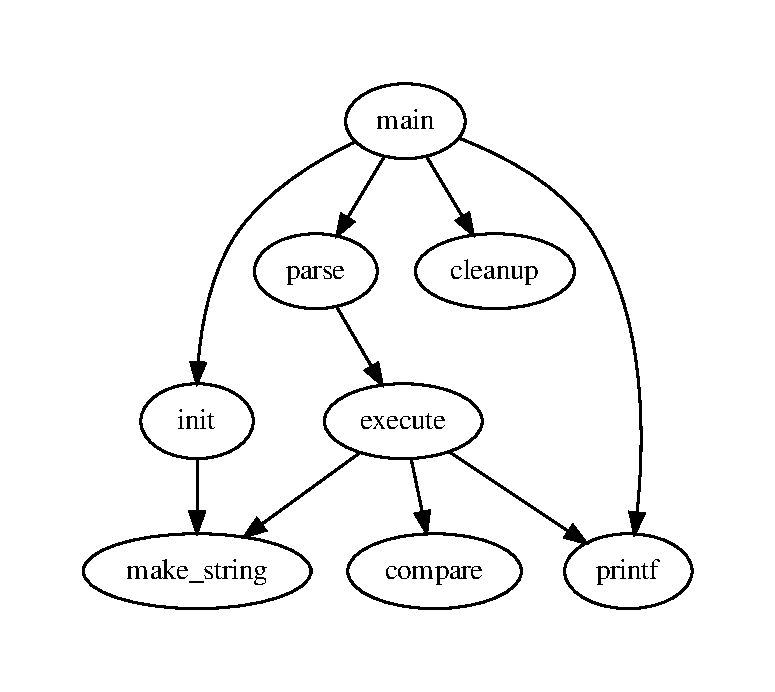
\includegraphics[width=\textwidth,height=\textheight/2,keepaspectratio=true]{dot_inline_dotgraph_25}}
\end{DoxyImageNoCaption}
 The command line option {\ttfamily -\/\+Tps} selects Post\+Script (E\+P\+SF) output. {\ttfamily small\+\_\+graph.\+ps} may be printed, displayed by a Post\+Script viewer, or embedded in another document.

Another useful tool based on {\ttfamily dot} is {\ttfamily dotty} which is a graph editor for the X Window System.\hypertarget{panda_sdk_graphviz_documentation}{}\subsection{Documentation}\label{panda_sdk_graphviz_documentation}
Documentation about Graph\+Viz and the D\+OT language can be found at \href{http://www.research.att.com/sw/tools/graphviz/refs.html}{\tt http\+://www.\+research.\+att.\+com/sw/tools/graphviz/refs.\+html} .\hypertarget{panda_sdk_graphviz_download}{}\subsection{Download}\label{panda_sdk_graphviz_download}
It is possible to download the last version of the Graph\+Viz tool both for Windows and Linux from the official website\+: \href{http://www.graphviz.org/pub/graphviz/CURRENT/}{\tt http\+://www.\+graphviz.\+org/pub/graphviz/\+C\+U\+R\+R\+E\+N\+T/}. \hypertarget{panda_sdk_graphviz_bibliography}{}\subsection{Bibliography}\label{panda_sdk_graphviz_bibliography}

\begin{DoxyItemize}
\item \mbox{[}E\+R\+G03\mbox{]} Emden R. Gansner, Drawing graphs with Graph\+Viz, 15 Aprile 2003.
\item \mbox{[}G\+N\+A00\mbox{]} E.\+R. Gansner and S.\+C. North. An open graph visualization system and its applications to software engineering. Software -\/ Practice and Experience, 30\+:1203-\/1233, 2000.
\end{DoxyItemize}\hypertarget{panda_sdk_doxygen_tag}{}\section{Doxygen}\label{panda_sdk_doxygen_tag}
{\ttfamily Doxygen} is a documentation system for C++, C, Java, Objective-\/C, I\+DL (Corba and Microsoft flavors) and to some extent P\+HP, C\# and D. It can help you in three ways\+:
\begin{DoxyItemize}
\item It can generate an on-\/line documentation browser (in H\+T\+ML) and/or an off-\/line reference manual (in LateX) from a set of documented source files. There is also support for generating output in R\+TF (M\+S-\/\+Word), Post\+Script, hyperlinked P\+DF, compressed H\+T\+ML, and Unix man pages. The documentation is extracted directly from the sources, which makes it much easier to keep the documentation consistent with the source code.
\item You can configure {\ttfamily doxygen} to extract the code structure from undocumented source files. This is very useful to quickly find your way in large source distributions. You can also visualize the relations between the various elements by means of include dependency graphs, inheritance diagrams, and collaboration diagrams, which are all generated automatically.
\item You can even `abuse\textquotesingle{} {\ttfamily doxygen} for creating normal documentation.
\end{DoxyItemize}

Doxygen is developed under Linux, but is set-\/up to be highly portable. As a result, it runs on most other Unix flavors as well. Furthermore, executables for Windows 9x/\+NT and Mac OS X are available.\hypertarget{panda_sdk_doxygen_download}{}\subsection{Download}\label{panda_sdk_doxygen_download}
Each Linux distribution provides Doxygen as developing tool, therefore before download it please check the web site check your distribution. The official W\+EB site is \href{http://www.doxygen.org/}{\tt http\+://www.\+doxygen.\+org/}.\hypertarget{panda_sdk_doxygen_documentation}{}\subsection{Documentation}\label{panda_sdk_doxygen_documentation}
Official documentation can be found at \href{http://www.doxygen.org/manual.html}{\tt http\+://www.\+doxygen.\+org/manual.\+html} .\hypertarget{panda_sdk_doxygen_panda_doc}{}\subsection{Documenting code in PandA}\label{panda_sdk_doxygen_panda_doc}
To know how to write a good documentation into PandA project, please see \hyperlink{documentation_how_to}{How To Create Good Documentation}. 